\Section{ETH. Нижние оценки про coloring'и}

\textit{Чем хороша \s{ETH}? Из неё вытекает оочень много условных нижних оценок на разные экспоненциальные задачи, например, на большинство задач из списка Карпа~\cite{Karp1972}. (Забавно, что это вообще не так для SETH: из всего большого списка только \s{Hitting Set} имеет условную нижнюю оценку под \s{SETH}). Единственная проблема \s{ETH} в том, что мы различаем с её помощью $2^{o(n)}$ и $2^{\Theta(n)}$, а между ними огромный зазор.}

\begin{remark}
    Для многих задач строится линейное сведение под \s{ETH} (например, число вершин в графе линейно относительно числа вершин/клозов). Для всех таких задач получаем оценку $2^{\Omega(n + m)}$.
\end{remark}

\subsection{\s{3-Coloring}}

\begin{problem}(\s{3-Coloring})
   Дан граф $G$. Можно ли его правильно раскрасить в 3 цвета.
\end{problem}

\begin{problem}(\s{Sparse 3-Coloring})
   Дан граф $G$, такой что $E(G) = \O(V(G)$. Можно ли его правильно раскрасить в 3 цвета.
\end{problem}

\begin{reduction}(\s{3-SAT} $\xto{2^{o(n)}, 2^{o(n + m)}}$ \s{Sparse 3-coloring})
    Создадим гаджет $K_3$, задающий 3 цвета: $T$, $F$ и $N$.

    Создадим по 2 вершины на каждую переменную $x_i$ и $\overline{x_i}$, соединим их с вершиной $N$ и друг с другом: так они будут принимать различные значения из $\{ T, F \}$.

    Опишем OR-гаджет ($x \vee y$): $K_3$, две вершины соединены с $x$ и $y$ соответственно, третья~--- выходная. Легко заметить, что она будет обязана быть покрашена в $F$ $\EQ$ $x$ и $y$ обе окрашены в $F$.

    Переменные каждого клоза соединим двумя OR-гаджетами, выходную вершину клоза соединим с $F$.

    Получаем 3 вершины для цветов, по 2 вершины на переменную и по 6 на каждый клоз. Рёбер тоже линейное число (поэтому получаем sparse инстанс).
\end{reduction}

\begin{problem}(\s{Planar 3-Coloring})
   Дан планарный граф $G$. Можно ли его правильно раскрасить в 3 цвета.
\end{problem}

\begin{fact}(Planar separator theorem)~\cite{Lipton1979}
    В планарном графе существует сбалансированный сепаратор (размер частей $\le \frac{2n}{3}$) размера $\O(\sqrt{n})$. Более того, его можно найти за линейное время.
\end{fact}

\begin{algorithm}{$2^{\O(\sqrt{n})}$ для \s{Planar List 3-Coloring}}\\
    Найдём сепаратор, переберём его раскраску. Решим \s{List 3-Coloring} для половинок. Итого $3^{\sqrt{n}} = 2^{\sqrt n}$
\end{algorithm}

\begin{remark}
    Часто, когда для задачи долго не получается придумать более быстрый алгоритм, оказывается, что это точная верхняя оценка. Так что сейчас мы покажем соответствующую нижнюю оценку для \s{Planar 3-Coloring}
\end{remark}

\begin{reduction}(\s{Sparse 3-Coloring} $\to$ \s{Planar 3-Coloring})

  \begin{adjustbox}{valign=T,raise=\strutheight,minipage={\linewidth}}
    \begin{wrapfigure}{r}{0.3\linewidth}
      \centering
      \vspace{-2.5em}
      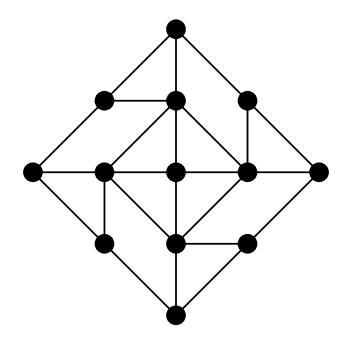
\includegraphics[scale=0.3]{02_crossover_gadget}
      \caption{Crossover gadget.}
      \label{img:crossover_gadget}
    \end{wrapfigure}

  \strut{}

  Построим гаджет, исправляющий пересечения рёбер (рис \ref{img:crossover_gadget}), при раскраске в 3 цвета цвета противоположных внешних вершин совпадают (и все пары раскрасок существуют). Воткнём такой гаджет на место каждого пересечения рёбер. Так как рёбер линейно от числа вершин.

\end{adjustbox} 

\end{reduction}

\begin{problem}(\s{$H$-coloring})\\
    Даны два графа $G$ и $H$, проверить, существует ли гомоморфизм из $G$ в $H$. 
    (гомоморфизм~--- отображение $g\colon G \to H$, т.ч. $\forall (u, v) \in E(G), (g(u), g(v)) \in E(H)$)\\

\end{problem}

\begin{remark}
\s{Coloring}~--- потому что если взять в качестве $H$ $k$-клику, получится просто \s{$k$-Coloring}. То есть мы красим вершины $G$ в цвета~--- вершины $H$~--- но не все пары цветов запрещены.
\end{remark}

\begin{remark}
Есть похожая задача~--- про миноры: проверить, что один граф является минором другого. И вот оказывается, что самым сложным минором является $k$-клика, её можно искать только за $k^{\Omega(k)}$.
\end{remark}

\begin{problem}(\s{$(2, k)$-CSP}) (Constraint satisfaction problem) \\
    Даны $n$ переменных, принимающих значения из алфавита размера $k$ и множество условий (предикатов) на двух переменных (любые условия, не только ДНФ).
\end{problem}

\begin{reduction}(\s{3-Coloring} $\xto{2^{\Omega(n)}, 2^{\Omega(n \log k)}}$ \s{$(2, k)$-CSP})\\
    По графу на $n$ вершинах построим $(2, k)$-CSP формулу на $\frac{n}{\log_3 k}$ переменных.\\
    Каждая переменная соответствует раскраске $\log_3 k$ вершин. А условия для каждой пары переменных запрещают противоречащие раскраски. Ну и понятно, нужно ещё запретить означивания переменных, в которых вершины из одного блока покрашены неправильно. 
\end{reduction}

\begin{statement}
\s{$H$-Coloring}~--- частный случай \s{$(2, k)$-CSP}.
\end{statement}

\begin{proof}
Означивание переменной соответствует ``цвету'' вершины. И единственные предикаты, которые можем использовать, задаются матрицей смежности $H$.\\
Заметим, что из этого факта вытекает, что \s{$3$-Coloring}~--- также частный случай \s{$(2, k)$-CSP}, в нём используется только предикат $\neq$.
\end{proof}

\begin{reduction}(\s{List $H$-Coloring} $\xto{2^{\Omega(n \log k)}, 2^{\Omega(n \log k)}}$ \s{$H$-Coloring}), где $k = |V(H)|$~\cite{Cygan2017} (скетч)\\
Пример: \s{List $3$-Coloring} $\to$ \s{$3$-Coloring}. Создадим треугольничек~--- ``палитру''~--- и соединим вершины, в которых запрещены какие-то цвета с соответствующими вершинами треугольничка.\\
Рассмотрим такой гаджет. Его понт в том, что при любом гомоморфизме центр переходит в центр. Чтобы работало и при большом $H$ (и не коллизилось с другими вершинами, засунем в центр клику $K_{k + 3}$).

\begin{figure}[H]
  \centering
  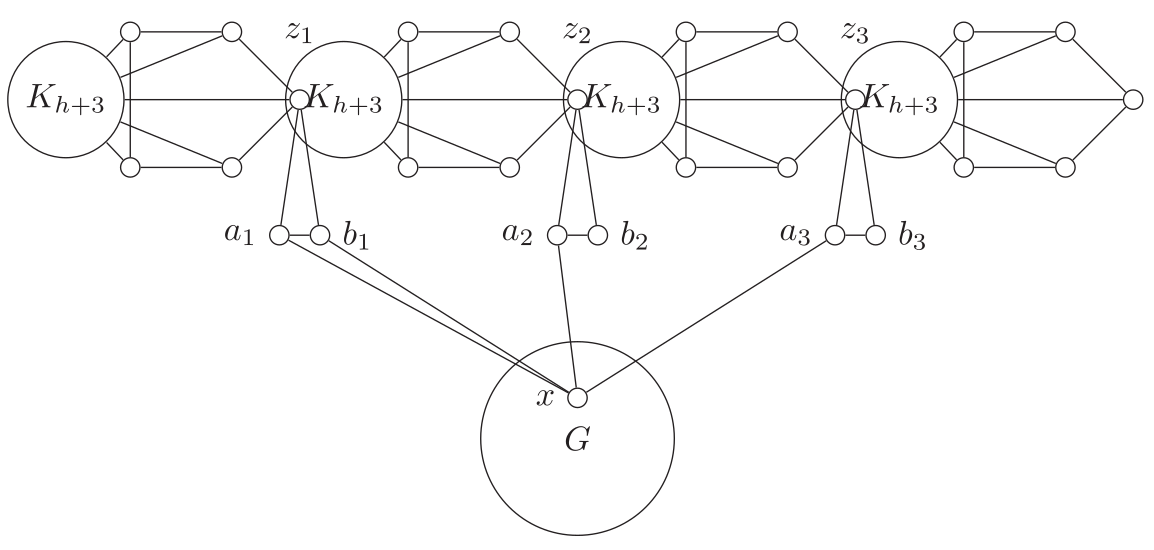
\includegraphics[scale=0.3]{02_list_h_coloring_gadget_worm}
  \caption{Пример гаджета для $k=3$, и вершины $x$, т.ч. $L(x) = \{1 \}$}
  \label{img:list_h_coloring_gadget_worm}
\end{figure}


Теперь сцепим $k$ таких гаджетов в цепочку. К каждому гаджету подвесим по две вершинки $a_i$ и $b_i$, это наша ``палитра''. Теперь вершинку графа $G$ соединим с $a_i$, и если её нельзя красить в $i$-ый цвет ещё и с $b_i$ (рис.~\ref{img:list_h_coloring_gadget_worm}). Аналогично соединяем с ``палитрой'' граф $H$. Примерно понятно, почему это работает (но тут скетч, так что строго не будет).


\end{reduction}


\begin{statement}\label{lm:lemma_3_2}~\cite{Cygan2017} 

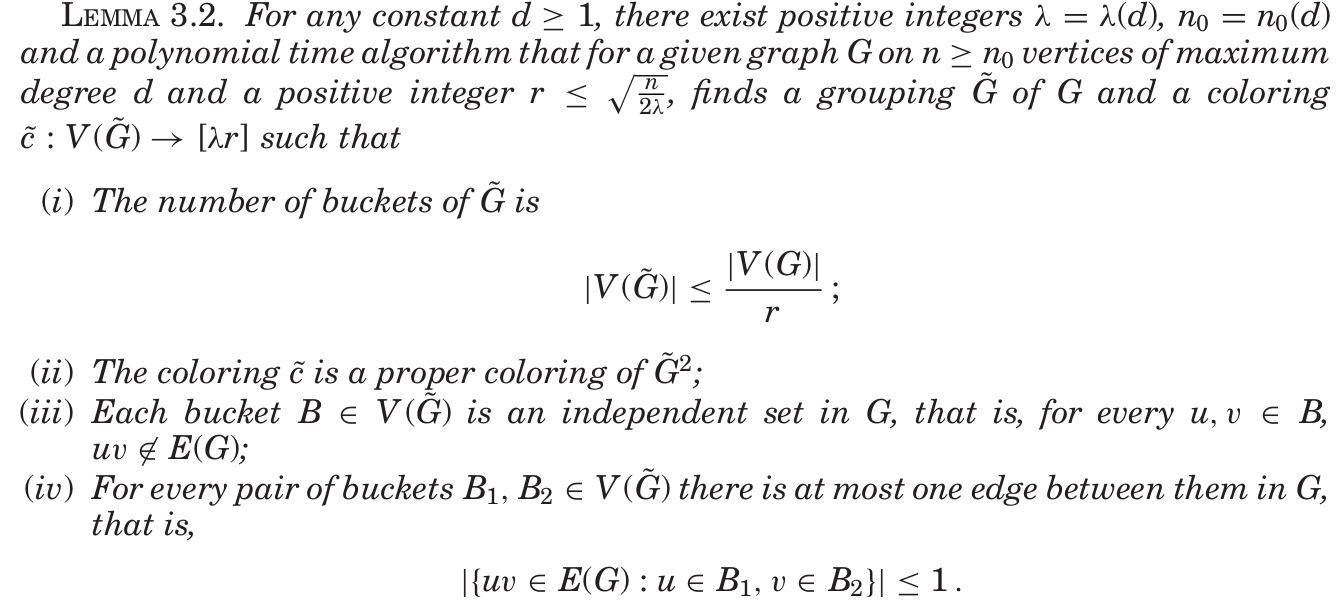
\includegraphics[scale=0.3]{02_lemma_3_2}
    
\end{statement}


\begin{reduction}(\s{Bounded Degree 3-Coloring} $\xto{2^{\Omega(n)}, 2^{\Omega(n \log k)}}$ \s{List $H$-Coloring}), где $k = |V(H)|$.\\

Хотим построить сведение примерно как для \s{$(2, k)$-CSP}~--- разбить вершинки на блоки, сжать блоки и решить \s{$H$-Coloring} для сжатого графа. Проблема в том, что мы не можем прослеживать связи между вершинами из разных блоков. Поэтому сведение будет более хитрым и потребует ``фактов из теории графов''.

Возьмём разбиение из утв.~\ref{lm:lemma_3_2} и его раскраску (будет говорить, что она задаёт не цвета, а лейблы, цвета~--- в исходном \s{3-Coloring}'е). Блоки образуют независимые множества и между двумя блоками не более одного ребра. Более того, так как раскраска переносится на $\widetilde{G}^2$, то для каждого блока все его соседи разных лейблов.

Для блока зададим 4-ичный вектор длины $\chi(\widetilde{G})$. На $t$-ой позиции этого вектора запишем цвет (в \s{3-Coloring}'е) соседа этого блока с лейблом $t$ (или 0, если такого нет). Тогда вершина в $H$ задаёт лейбл блока и кодировку. \s{List $H$-Coloring}'ом (частью про \s{List}) добиваемся того, что блок отображается только в свой лейбл. Соединяем в $H$ вершины, раскраски которых согласованы ($\phi_a (b) \neq \phi_b (a) \vee \phi_a (b) \phi_b (a) = 0$).

Теперь оценим время. Выберем размер блока равным $r$, тогда $|V(\widetilde{G})| \le \frac{n}{r}$, $|V(H)| \le \chi(\widetilde{G}) 4^{\widetilde{G}} = \O(r 4^{\O(r)})$. Выбрав $r = \O(\log n)$ получаем $|V(G)| = \O(\frac{n}{\log n})$, $|V(H)| = n^{\O(1)}$.

\end{reduction}

\begin{problem}(\s{Subgraph Isomorphism})
Даны графы $G$ и $H$, проверить, является ли $H$ подграфом $G$.
\end{problem}

\begin{reduction}(\s{$H$-Coloring} $\xto{2^{\Omega(n \log n)}, 2^{\Omega(n \log n)}}$ \s{Subgraph Isomorphism})\\
Переберём $a_i, \sum\limits_{i=1}^{|V(H)|} a_i = |V(G)|$~--- сколько вершин $G$ отобразится в $i$-ую вершину $H$. Продублируем $i$-ую вершину $H$ $i$ раз, поищем изоморфизм из $H$ в $G$. Так как неупорядоченных разбиений на слагаемые будет не более $2^{|V(G)|} = 2^{n}$ получили нужную оценку.

\end{reduction}

\subsection{Семинар}

\begin{exerc}
    $\forall \alpha > 0$ построить $(2^n, n^{1 + \alpha})$ fg-сведение \s{Ham Cycle} $\to$ \s{3-Sum}
\end{exerc}

\begin{problem}(\s{Max Inner Product})\\
    Даны $2$ набора $A$ и $B$ из $n$ векторов из $\{0, 1\}^d$, где $d = o(n)$. Найти $\max \{ \langle a, b \rangle | a \in A, b \in B \}$.
\end{problem}
    
\begin{exerc}
    Покажите, что \s{Max Inner Product} не решается за время $\O(n^{2 - \eps})$ под \s{SETH}.
\end{exerc}

\begin{exerc}
    Покажите оценку в $2^{\Omega(n)}$ на \s{Bounded Degree 3-Coloring} ($\frac{|E(G)|}{|V(G)|} = n^{o(1)}$) под \s{ETH}.
\end{exerc}
% просто есть сведение с degree <= 4

\begin{problem}(\s{Cross Matching})
    Дан граф $G$ с разбиением вершин на две доли по $n$ вершин. Проверить, существует ли такое совершенное паросочетание $M$ в $G$, что концы каждого ребра паросочетания находятся в разных долях и $G/M$ (стянутые рёбра) образует клику.
\end{problem}

\begin{exerc}\cite{Fomin2021}
    Покажите оценку в $n^{\Omega(n)}$ на задачу \s{Cross Matching} под \s{ETH}.
\end{exerc}



